\documentclass{article}
\usepackage[utf8x]{inputenc}
\usepackage[francais]{babel}
\usepackage[T1]{fontenc}
\usepackage[autolanguage,np]{numprint}
\usepackage{boxedminipage}

\usepackage{Sweave}
\begin{document}
\Sconcordance{concordance:samu.tex:samu.Rnw:%
1 7 1 1 0 2 1 1 31 19 1 1 23 15 0 1 10 1 2 2 1 1 9 1 2 3 1 1 9 10 1 1 %
14 1 2 1 3 1 2 3 1 1 9 1 2 2 1 1 8 13 0 1 2 1 1}



\section*{Activité des SAMU alsacien}

Les données proviennent du serveur régional SAGEC. Les informations sont transmises au serveur par les deux SAMU, sur la base des informations demandées par l'ARH en 2005, sous forme d'une synthèse quotidienne:
\begin{itemize}
  \item date
  \item nombre d'affaires régulées
  \item nombre d'interventions primaires
  \item nombre d'interventions secondaires
  \item nombre de transport de néonatalogie
  \item nombre de transfert infirmier inter hospitaliers
  \item nombre de transports par ambulances privées demandés par le SAMU
  \item nombre de transport par VSAV demandés par le SAMU
  \item nombre de conseils médicaux
  \item nombre de visites de médecins déclenchées par le Centre 15
\end{itemize}
La base de données est renseignées depuis le mois de juillet 2005. En 2012, une difficulté au niveau de l'hôpital de Mulhouse a entraîné un arrêt complet des transmissions pendant 6 mois en en 2013, une erreur logicielle à provoqué la transmissions de données erronées en provenance du SAMU 67 du 24 avril au 1er novembre 2013. Les données 2013 sont globalement sous estimées.

Le interventions SMUR sont égales à la somme des interventions primaires et secondaires.

% latex table generated in R 3.0.2 by xtable 1.7-1 package
% Wed Jan 15 18:35:54 2014
\begin{table}[ht]
\centering
\begin{tabular}{rrrrrrrrr}
  \hline
 & 2006 & 2007 & 2008 & 2009 & 2010 & 2011 & 2012 & 2013 \\ 
  \hline
Affaires & 394904 & 431340 & 432576 & 446044 & 429529 & 412890 & 414947 & 417157 \\ 
  Conseils & 86124 & 79961 & 81572 & 94640 & 84969 & 77585 & 58646 & 87921 \\ 
  SMUR & 25547 & 25625 & 25766 & 26545 & 25015 & 23214 & 22724 & 24494 \\ 
  ASSU & 57243 & 63190 & 61788 & 40807 & 46350 & 44360 & 42366 & 42167 \\ 
  VSAV & 22779 & 23379 & 29168 & 33984 & 33238 & 29169 & 25213 & 40281 \\ 
  Médecins & 55588 & 67981 & 69448 & 74293 & 65509 & 59062 & 48704 & 53820 \\ 
   \hline
\end{tabular}
\end{table}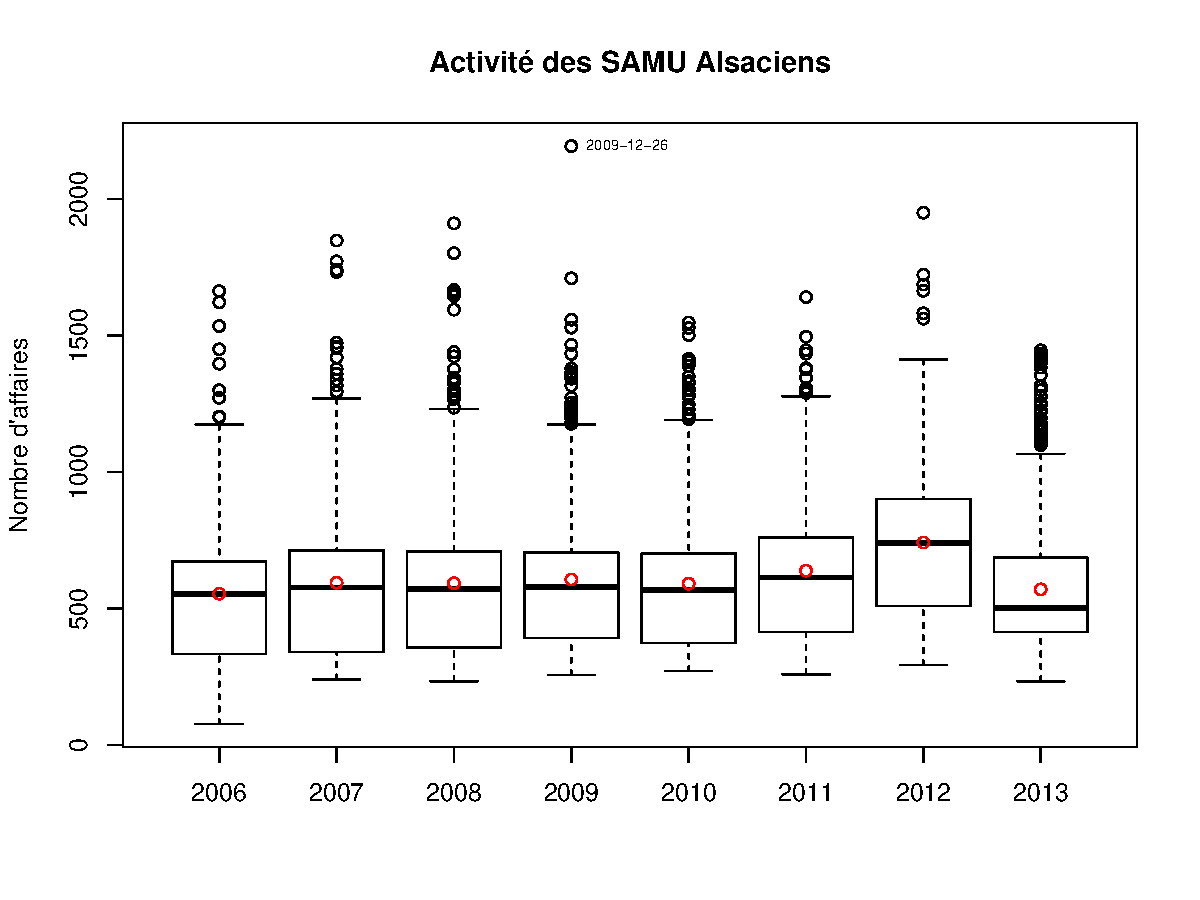
\includegraphics{samu-global}

Après une période de stabilité (2006-2011), l'activité augmente à nouveaux à partir de 2011.

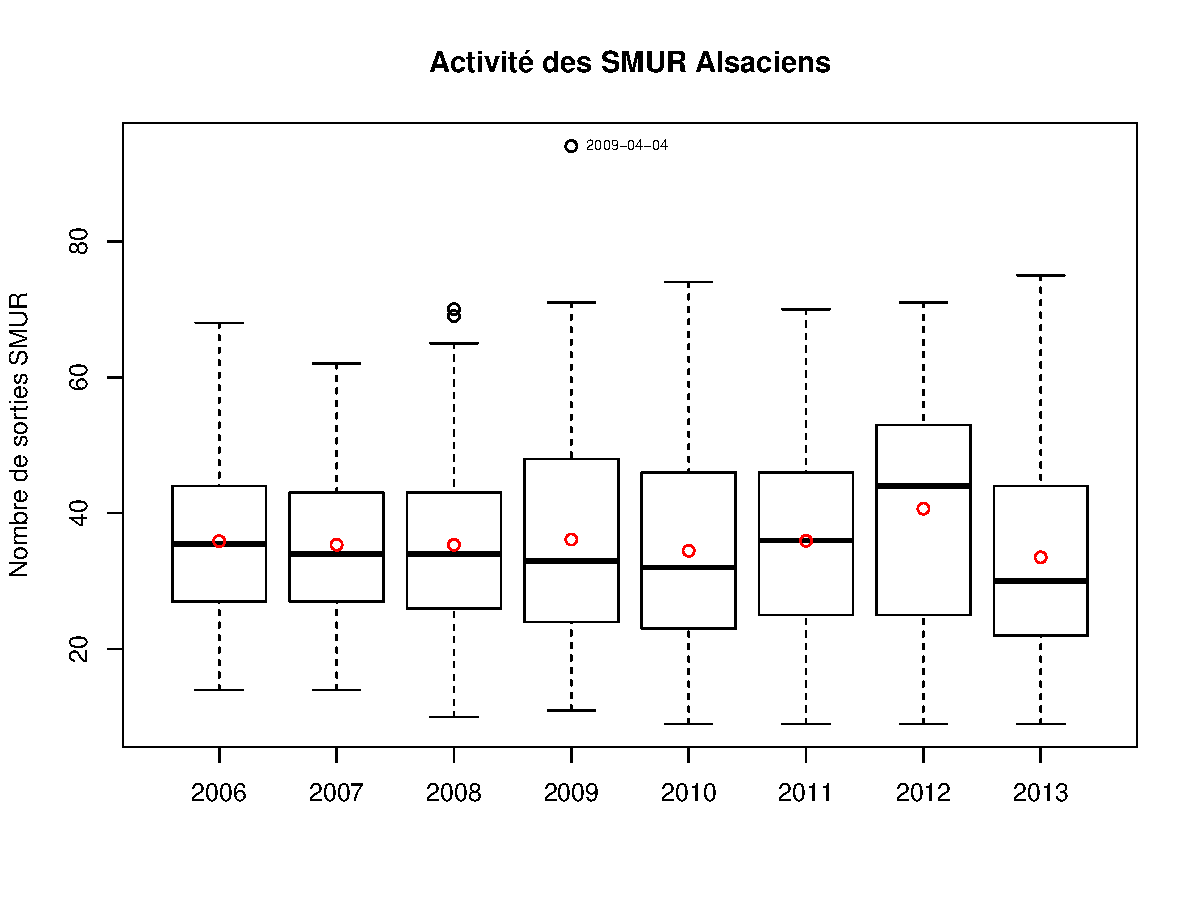
\includegraphics{samu-smur}


\section*{Activité des SAMU alsacien en 2013}


\begin{boxedminipage}{10cm}
\begin{itemize}
  \item nombre d'affaires: \np{2260} pour \np{10000} habitants.
  \item nombre de sorties SMUR: \np{133} pour \np{10000} habitants.
  \item nombre de conseils médicaux: \np{476} pour \np{10000} habitants.
  \item nombre d'envoi de médecins:  \np{292} pour \np{10000} habitants.
\end{itemize}
\end{boxedminipage}


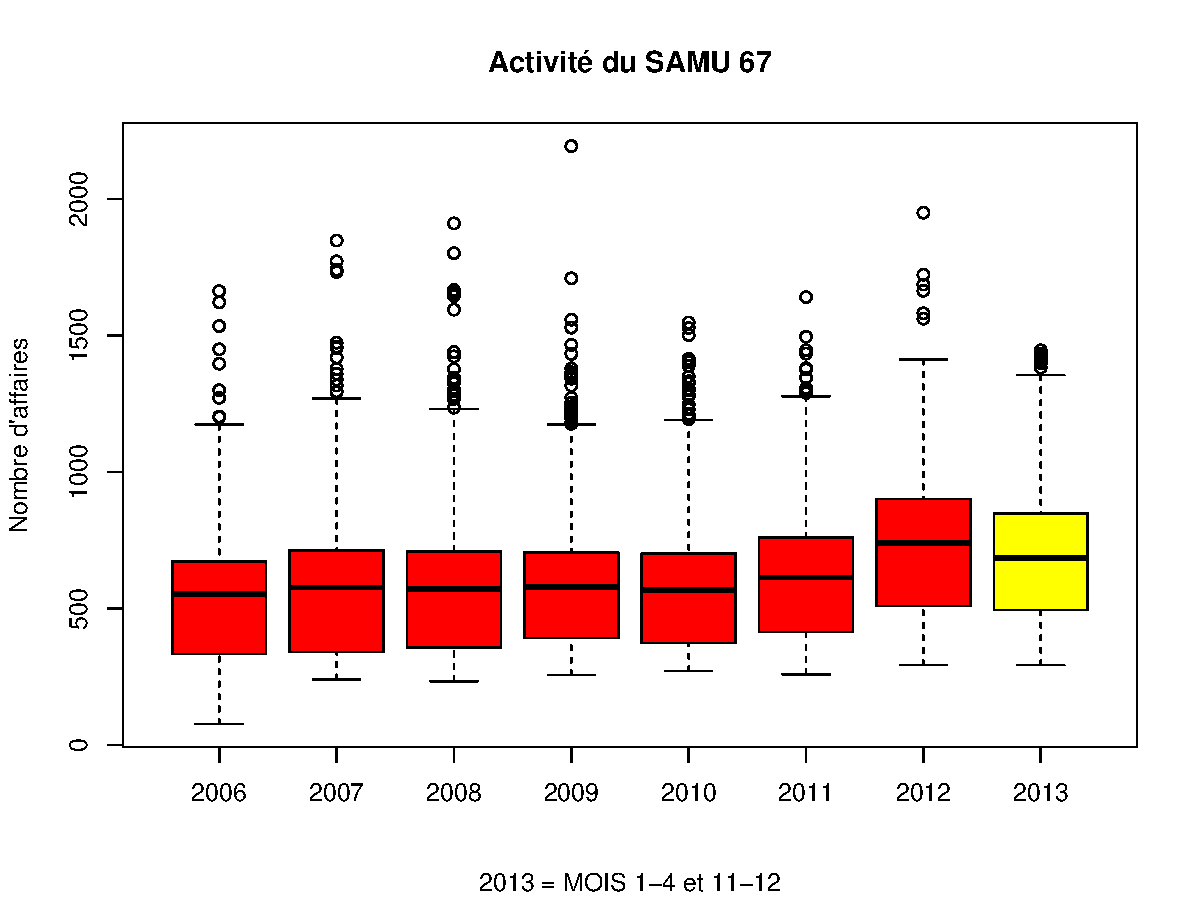
\includegraphics{samu-samu67}

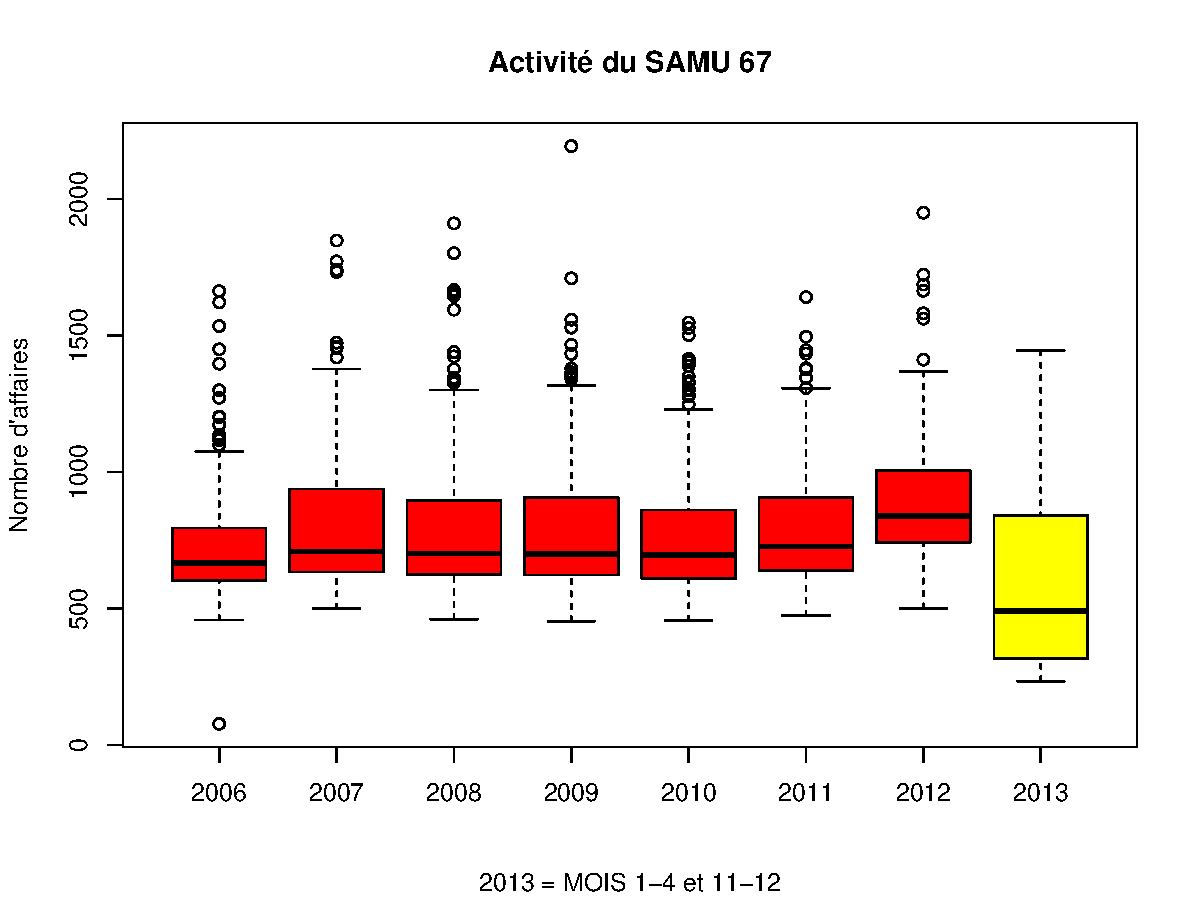
\includegraphics{samu-samu67_2}


Activité comparée des deux SAMU

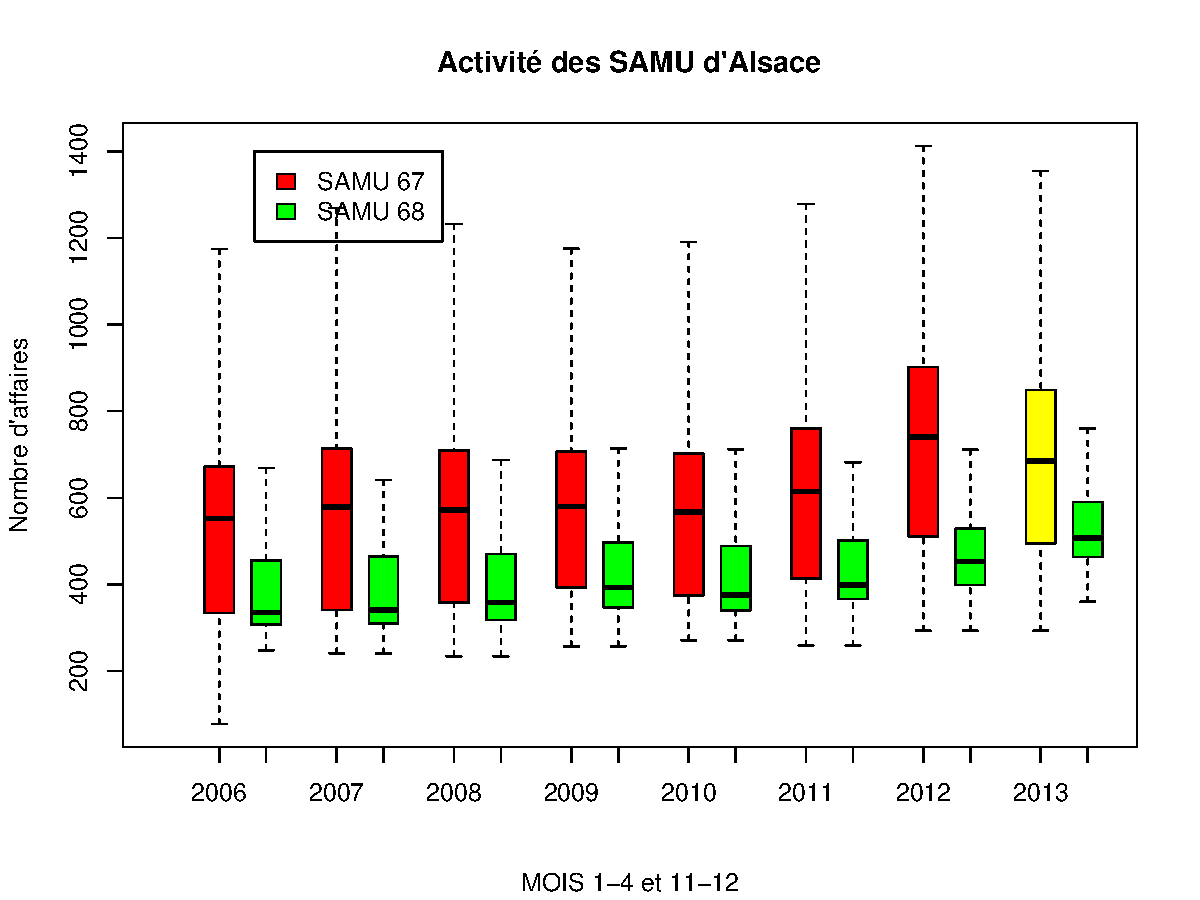
\includegraphics{samu-samu6768}

L'activité du SAMU 67 est élevée avec un taux de recours de l'ordre de 25\%. Le SAMU 68 a une activité inférieure à celle du SAMU 67 mais connait une croissance très forte ces dernières années qui a fait progresser de façon marquée son taux de recours.
\index{SAMU!taux de  recours}
% latex table generated in R 3.0.2 by xtable 1.7-1 package
% Wed Jan 15 18:35:54 2014
\begin{table}[ht]
\centering
\begin{tabular}{rrrrrrrrr}
  \hline
 & 2006 & 2007 & 2008 & 2009 & 2010 & 2011 & 2012 & 2013 \\ 
  \hline
67 & 23.55 & 26.58 & 26.26 & 26.18 & 25.51 & 26.52 & 29.53 & 20.39 \\ 
  68 & 18.25 & 18.68 & 19.32 & 20.58 & 20.00 & 16.31 & 12.18 & 25.72 \\ 
   \hline
\end{tabular}
\caption[Taux de recours des SAMU]{Taux de recours des SAMU 67 et 68. Si le taux de recours du SAMU 68 est plus faible que celui du SAMU 67, il connait une forte progression (les années 20122 et 2012 sont incomplètes pourle 68).} 
\label{fig.rec}
\end{table}
\end{document}
